\documentclass[a4paper,12pt]{article}

\usepackage[T1]{fontenc}
\usepackage{times}
\usepackage[swedish,english]{babel}
\usepackage[utf8]{inputenc}
\usepackage{dtklogos}
\usepackage{wallpaper}
\usepackage[absolute]{textpos}
\usepackage[top=2cm, bottom=2.5cm, left=3cm, right=3cm]{geometry}
\usepackage{appendix}
\usepackage[nottoc]{tocbibind}
%\usepackage{setspace}

\setcounter{secnumdepth}{3}
\setcounter{tocdepth}{3}

\usepackage{sectsty}
\sectionfont{\fontsize{14}{15}\selectfont}
\subsectionfont{\fontsize{12}{15}\selectfont}
\subsubsectionfont{\fontsize{12}{15}\selectfont}

\usepackage{csquotes} % Used to handle citations
\renewcommand{\thetable}{\arabic{section}.\arabic{table}}  
\renewcommand{\thefigure}{\arabic{section}.\arabic{figure}}

%----------------------------------------------------------------------------------------
%	
%----------------------------------------------------------------------------------------
\newsavebox{\mybox}
\newlength{\mydepth}
\newlength{\myheight}

\newenvironment{sidebar}%
{\begin{lrbox}{\mybox}\begin{minipage}{\textwidth}}%
{\end{minipage}\end{lrbox}%
 \settodepth{\mydepth}{\usebox{\mybox}}%
 \settoheight{\myheight}{\usebox{\mybox}}%
 \addtolength{\myheight}{\mydepth}%
 \noindent\makebox[0pt]{\hspace{-20pt}\rule[-\mydepth]{1pt}{\myheight}}%
 \usebox{\mybox}}

%----------------------------------------------------------------------------------------
%	Title section
%----------------------------------------------------------------------------------------
\newcommand\BackgroundPic{
    \put(-2,-3){
    
\includegraphics[keepaspectratio,scale=0.3]{img/lnu_etch.png} % Background picture
    }
}
\newcommand\BackgroundPicLogo{
    \put(30,740){
    
\includegraphics[keepaspectratio,scale=0.10]{img/logo.png} % Logo in upper left corner
    }
}

\title{	
\vspace{-8cm}
\begin{sidebar}
    \vspace{10cm}
    \normalfont \normalsize
    \Huge Assignment 1: Jodel Alert Design Document\\
    \vspace{-1.3cm}
\end{sidebar}
\vspace{3cm}
\begin{flushleft}
    \huge Software Engineering - Design\\ 
    \it \LARGE - 2DV603
\end{flushleft}
\null
\vfill
\begin{textblock}{6}(10,12)
\begin{flushright}
\begin{minipage}{\textwidth}
\begin{flushleft} \large
\emph{Name:} Patrik Hermansson\\ % Author
\emph{Email:} ph222md@student.lnu.se\\
\emph{Name:} Michael Wagnberg\\ % Author
\emph{Email:} mw222uu@student.lnu.se\\
\emph{Name:} Benjamin Svärd\\ % Author
\emph{Email:} bs222et@student.lnu.se\\
\emph{Name:} Christofer Nguyen\\ % Author
\emph{Email:} cn222hn@student.lnu.se\\
\emph{Name:} Jonathan Walkden\\ % Author
\emph{Email:} jw222qi@student.lnu.se\\
\end{flushleft}
\end{minipage}
\end{flushright}
\end{textblock}
}

\date{} 
\newpage
\begin{document}
\pagenumbering{gobble}
\newgeometry{left=5cm}
\AddToShipoutPicture*{\BackgroundPic}
\AddToShipoutPicture*{\BackgroundPicLogo}
\maketitle
\restoregeometry
\selectlanguage{english}
\pagenumbering{gobble}
\newpage
\tableofcontents % Table of contents
\pagenumbering{arabic}
\newpage
\section{Design Document}
\subsection{Purpose}
This document will describe the entire design and decisions as well as  rationales regarding Jodel application API, work-arounds, client-server and core functionality and vital parts of Jodel Alert.\\

The Jodel Alert Application will scan Jodel post feed, derive keywords desiderata and notify an email recipient(requirement ID 1). It will do this every 15 minutes (requirement ID 2). Possible failure conditions can be that Jodel Alert will not get an authenticated token, the server which Jodel Alert runs upon is down, or wrong format of email recipient. This will be handled by error messages to the user.\\

The Jodel Alert Application user will be able to add and change email recipient as well as keywords(requirement ID 4,5,6,7)\\

The Jodel Alert Application admin will be able to remove email recipient and keywords(requirement 3,8) as well as the ordinary user actions.\\




\subsection{General priorities}
One of our highest priorities is simplicity. The core problem we are trying to solve, the project idéa, is in itself simple and small, which makes it reasonable to design everything with simplicity in our minds.\\

The alert that raises awareness of a post that Linnéstudenterna is interested in is the important result. There are several ways to accomplish that, you can have an advanced GUI for the customer, or different ways to change the properties of keywords and email. 
 
We have designed everything to just solve the core problem, the alert. The Jodel Alert will run in the background on a server, and send alerts (emails) when keywords found. \\

We have also focused on reuseability as a priority in our design, this is merely because of our projects uniqueness on the Jodel application. \\

Everything will be general and not suited just for our customer, this makes other companies potential customers.\\

To get our application to have high scalability, we decided to make a user and administrator mode.
With the case of just a generic user that can change, add and remove keywords and email recipients works fine for a smaller business with maybe 5-10 employees.
To ensure scalability we decided that we had to implement an administrator and a user system. This means that a bigger company can have a few administrators that have more privileges than the other users, which in turn results in a better maintained database of keywords and emails.\\

We also wanted to design for portability. The application will be written and developed in Java. This makes it versatile, supported by multiple vendors and can work on all platforms needed.


\subsection{Design issues}
One of the first things that had to be resolved was of course the Jodel API. We did not know if that API was open or not accessible for the general public. We planned accordingly to cover both situations, so we were ready to design with the API or without. \\

After several tries of contacting the developers of Jodel we understood that no answer would arrive. Instead we moved towards a program called mitmproxy, that deals with listening to the traffic from Jodel by imitating an ordinary client cellphone. We can then extract that data and use it in our favour.\\
Choosing database was another possible constraint or issue. Regarding to the technical aspect, maybe no one in the group have competence to use a powerful database (like MySQL) in collaboration with the never used program mitmproxy. Another aspect is budget and time for implementing MySQL as a database.  \\

We have choosen a design that fits a "database", and we can easily choose between a commercial database or just a plane text file, depending on difficulties and other constraints that may show up.\\


\subsection{Outline of the design}
(Probably not in the finished version)?
\clearpage
\section{Design details}
The UML use cases describe the systems behaviour and what each case intends to achieve. This UML design phase is implemented to achieve for both stakeholders and project members an understanding for how the applications functions will work together with the end-user.  \\

Following in this section there will also be a graphical illustration of the use cases depict in workflows that will be intended to describe the operational workflows of the system. To view activity diagram look on appendix 1.2.\\

All key components for this application is listed here.\\
\subsection{Activity diagram - Handle Jodel Post}
\begin{figure}[!h]
	\centering
	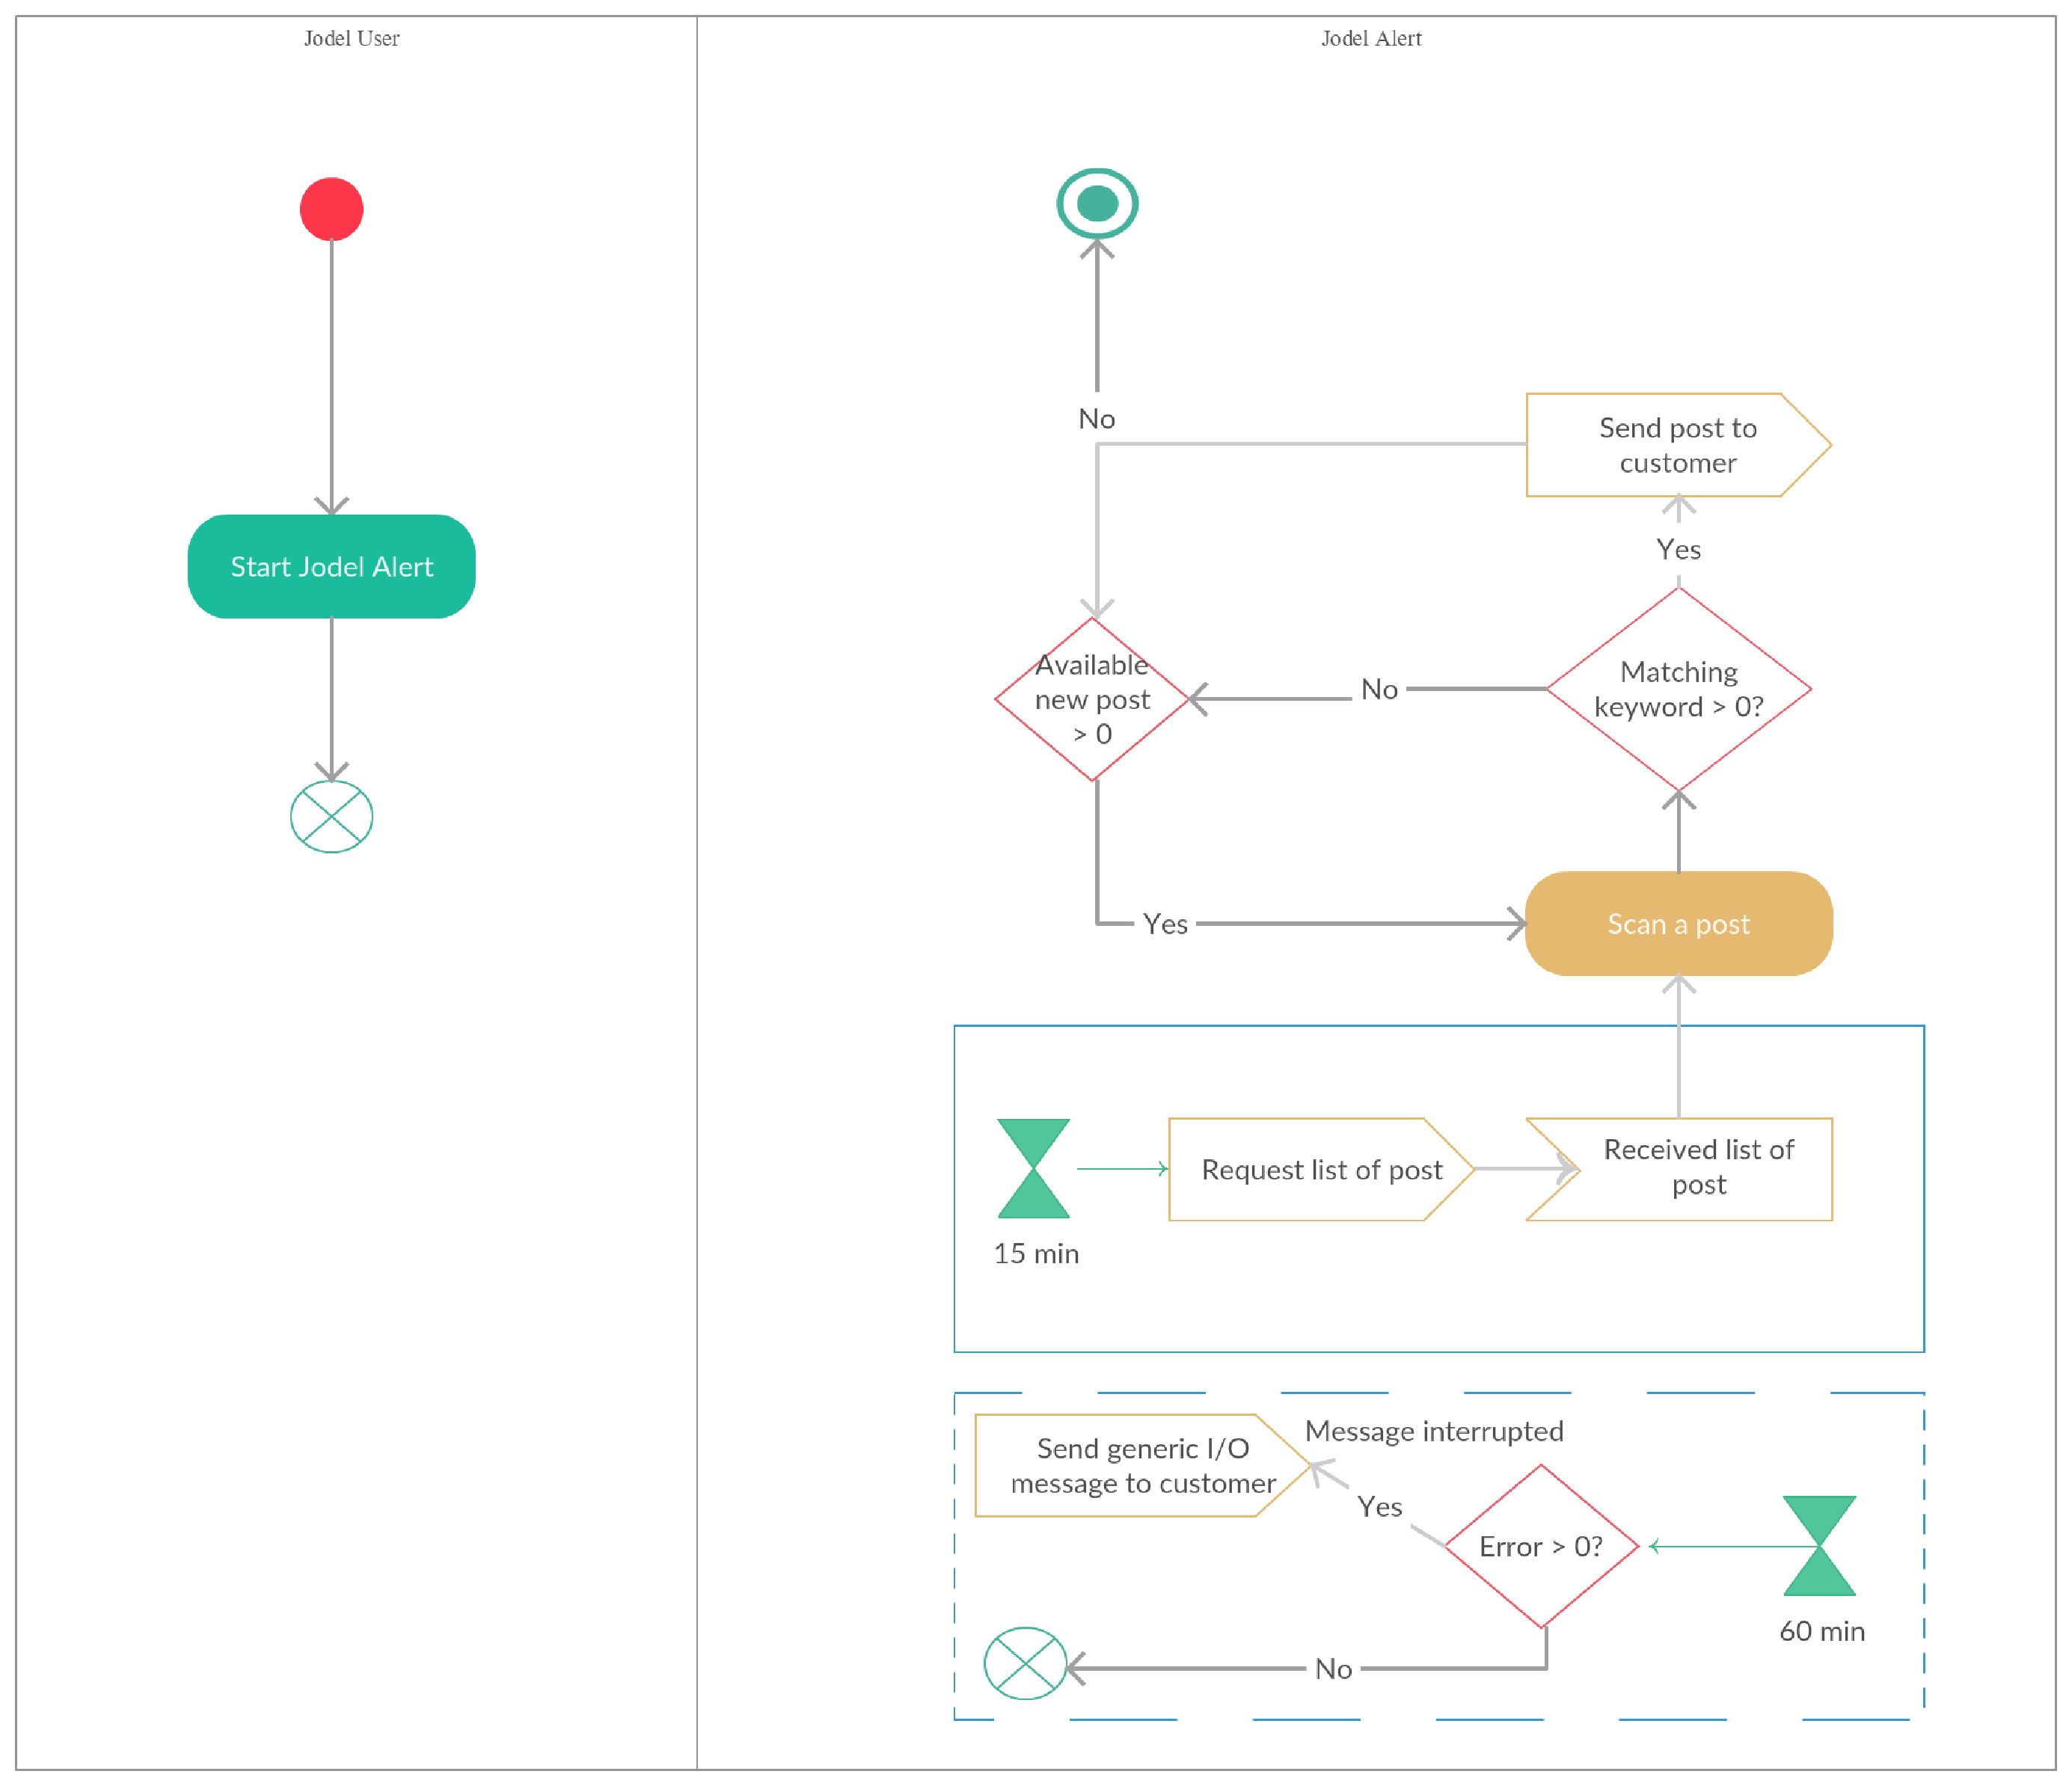
\includegraphics[height=13cm]{img/Activity_diagram-Handling_Jodel_post.pdf}
	\caption{Jodel Alert Activity Diagram Handling Jodel Post}
	\label{Jodel}
\end{figure}
\clearpage
\subsection{Activity diagram - Modifying Database}
\begin{figure}[!h]
	\centering
	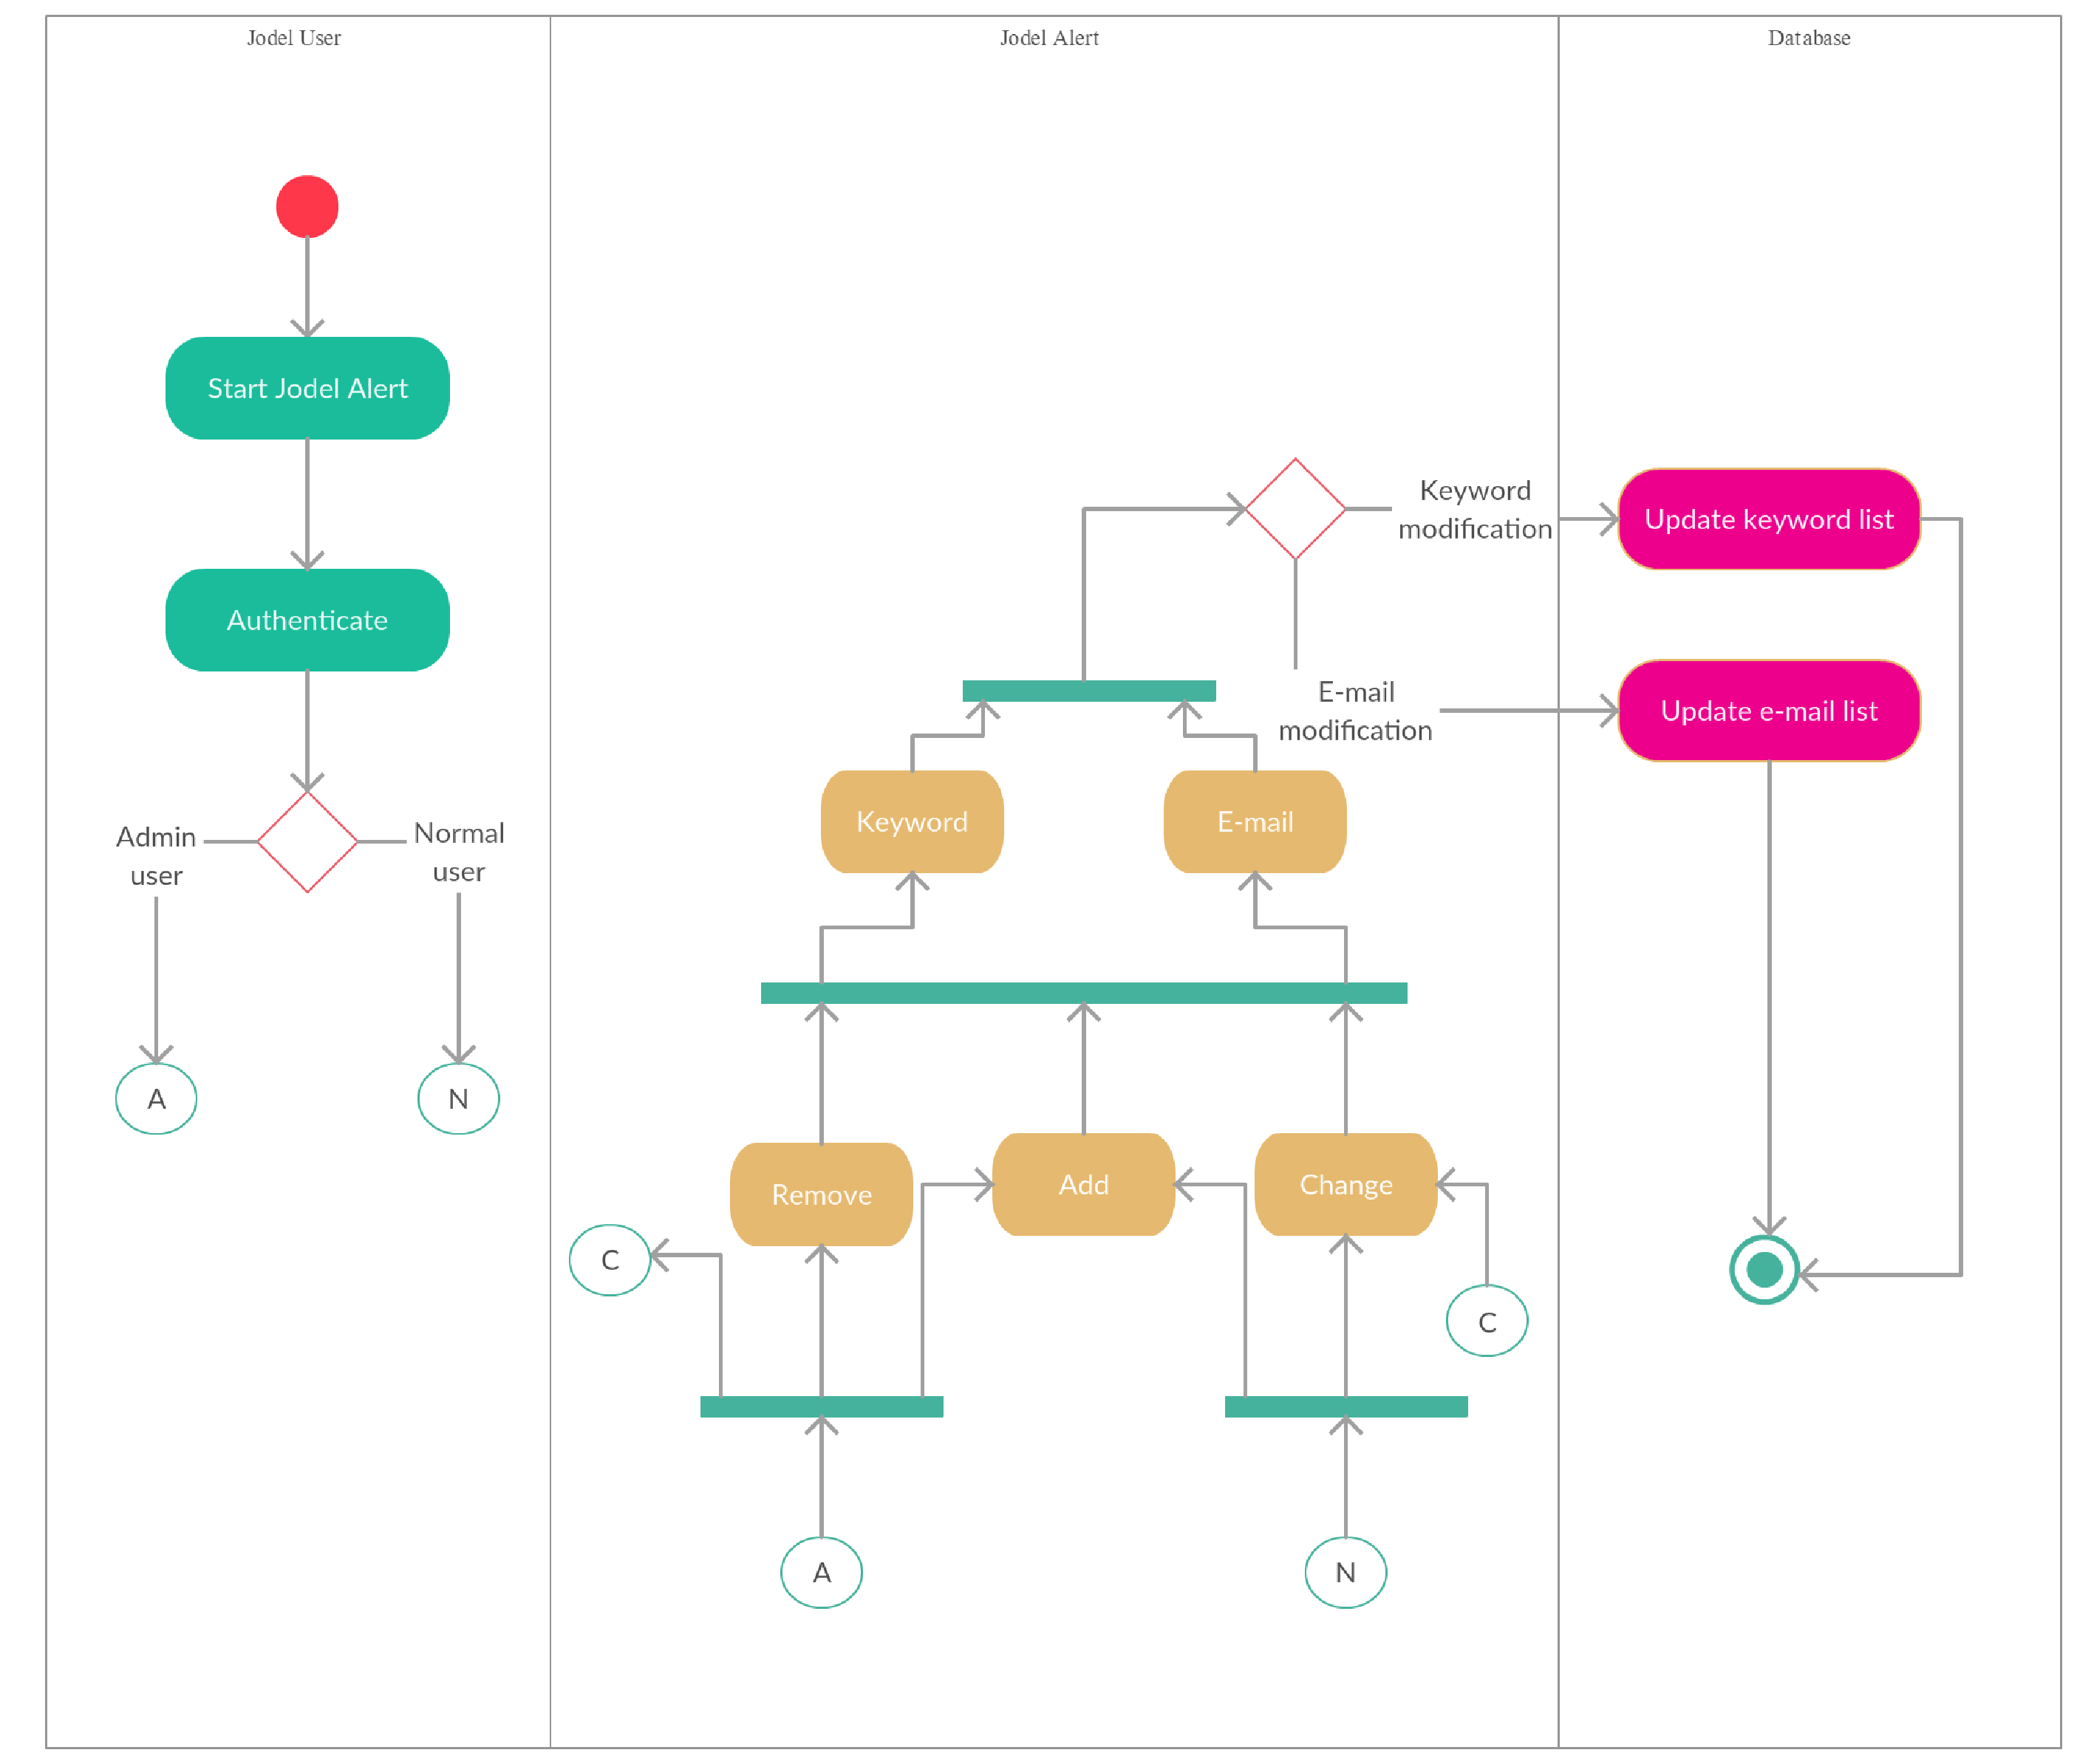
\includegraphics[height=13cm]{img/Activity_diagram-Modifying_database.pdf}
	\caption{Jodel Alert Activity Diagram Modifying Database}
	\label{Jodel}
\end{figure}
\clearpage
\subsection{Constraints}
(Probably not in the finished version)?
\subsection{Design options}
\begin{figure}[!h]
	\centering
	\includegraphics[height=6cm]{img/designspace.pdf}
	\caption{Jodel Alert Design Space}
	\label{Jodel}
\end{figure}
User interface vs no user interface is a big difference. As we stated in requirement ID 13 the user interface should be easy to use and simple. If going for no user interface the users are forced to have a higher level of knowledge to operate the application correctly. Adding a simple keyword can mean knowledge of how databases works and maybe require other programs. With the user interface the user can add a simple keyword without knowing about the underlying backbone of our system.
This gives the application good usability.\\

We choose an SQL database which is easier to maintain, than a plane text file. We also get the properties of using Jodel Alert Application on several machines on work and at home, which does not work if using a text file locally on the machine running the application.
Scalability is also reached with using an SQL database.\\

One of the design issues mentioned before was the use of the Jodel API. This was not open and accessible for the general public, and we did not get any response from the Jodel company. This forced us to choose the path of no API at all.
\clearpage
\section{Risk mitigation}
(Probably not in the finished version)?
\section{Class diagram}
\begin{figure}[!h]
	\centering
	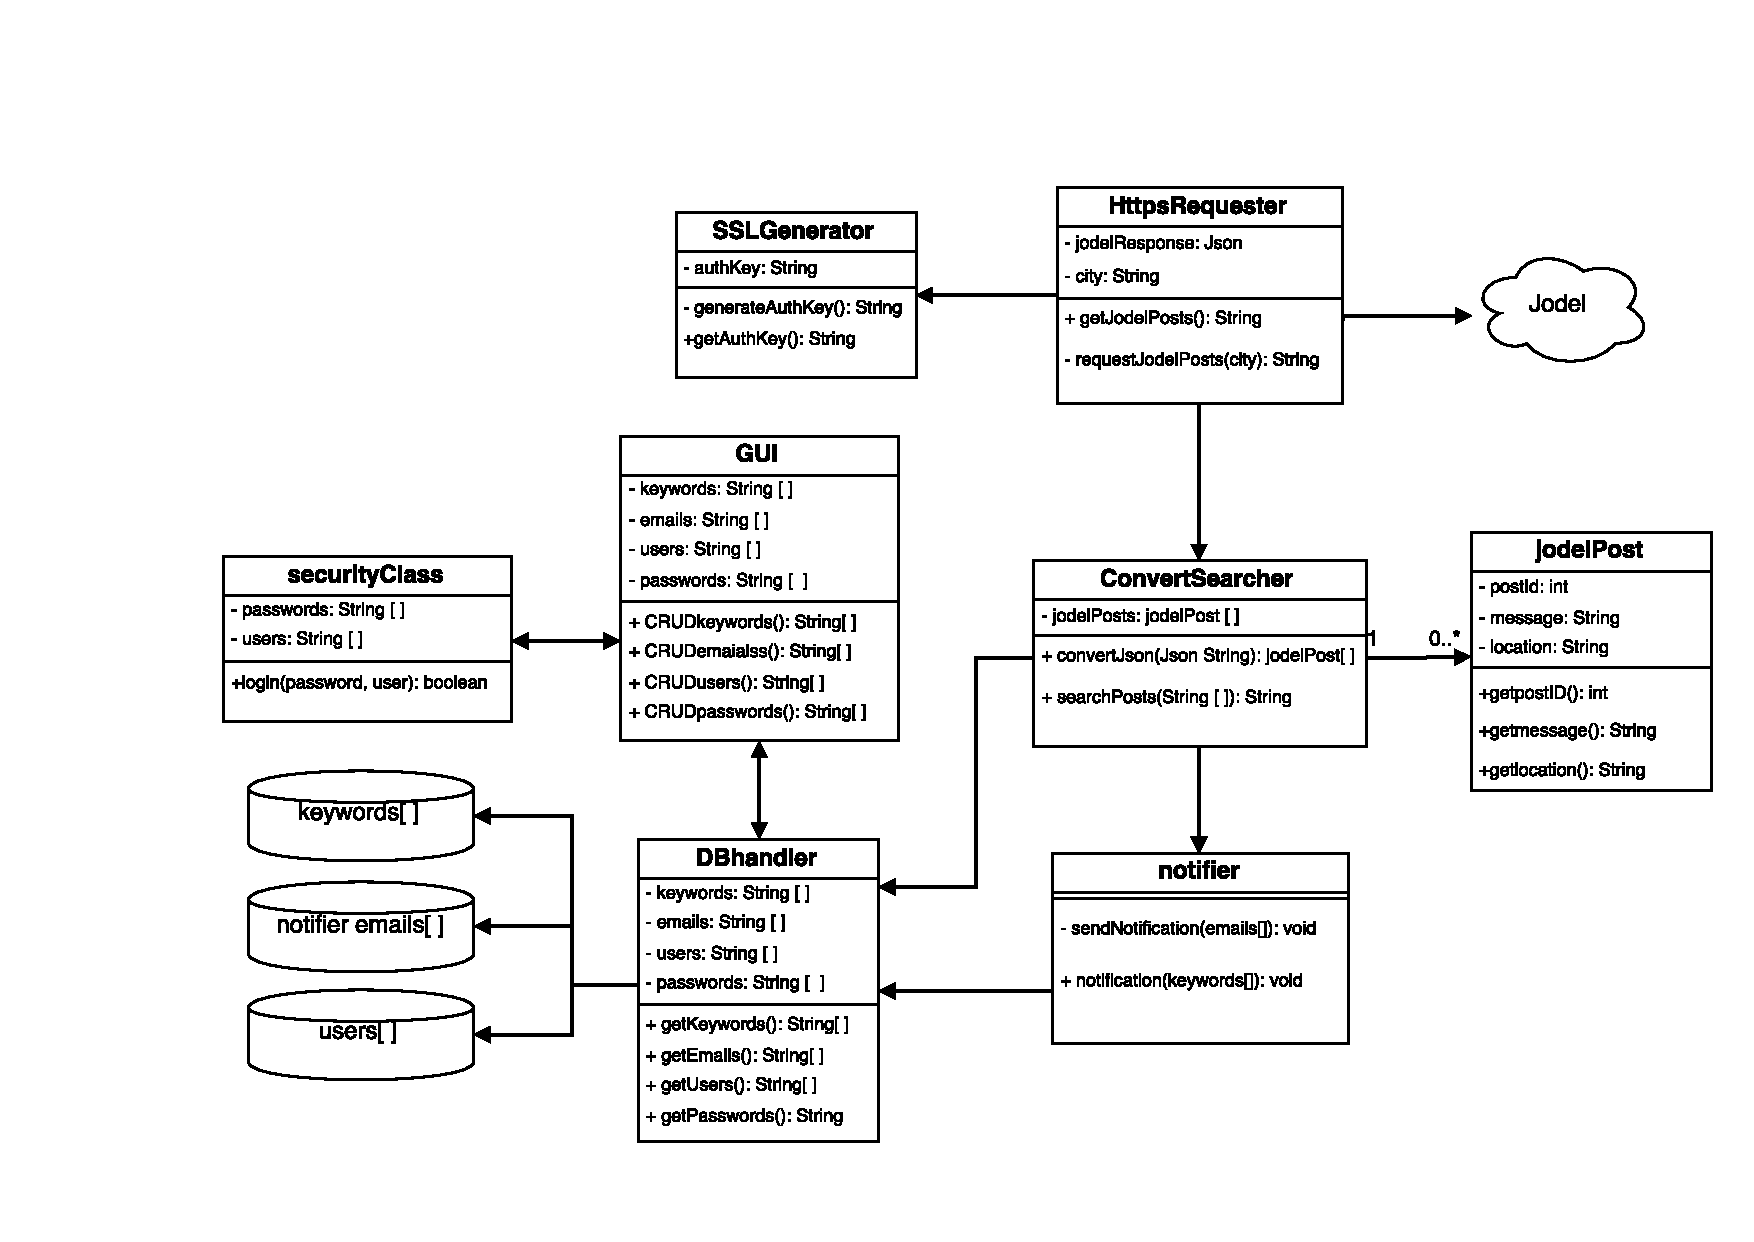
\includegraphics[height=12cm]{img/jodelUMLClassDiagram.pdf}
	\caption{Jodel Alert Class Diagram}
	\label{Jodel}
\end{figure}
\clearpage
\section{Component Diagram}
\begin{figure}[!h]
	\centering
	\includegraphics[height=11cm]{img/component_diagram.pdf}
	\caption{Jodel Alert Component Diagram}
	\label{Jodel}
\end{figure}
\clearpage
\section{Sequence Diagram}
\begin{figure}[!h]
	\centering
	\includegraphics[height=13cm]{img/sequence_diagram1.pdf}
	\caption{Jodel Alert Sequence Diagram}
	\label{Jodel}
\end{figure}
\clearpage
\begin{figure}[!h]
	\centering
	\includegraphics[height=13cm]{img/sequence_diagram2.pdf}
	\caption{Jodel Alert Sequence Diagram}
	\label{Jodel}
\end{figure}
\clearpage
\section{After release}
Some things is always forced to be omitted because of time, budget and other constraints.\\

In version 2.0 of our application we would like to develop the following features:
\begin{itemize}
	\item Ability to post answers to Jodel directly from the GUI of Jodel Alert
	\item Each user can have their own customized keywords
\end{itemize}
\begin{figure}[!h]
	\centering
	
\includegraphics[height=6cm]{img/jodel.png}
	\caption{Jodel logo}
	\label{Jodel}
\end{figure}

\end{document}